\section{Processo de implementação do algoritmo KNN em VHDL}

O algoritmo usado na implementação VHDL foi o KNN pela distancia euclidiana. 
Esta é a distância entre dois pontos, que pode ser provada pela aplicação
repetida do teorema de Pitágoras \cite{wiki:ieee754en}. A distancia euclidiana
entre o ponto P($p_1, p_2, p_3, ..., p_n$) e Q($q_1, q_2, q_3, ..., q_n$) é
dada por:

$d(p, q) = \sqrt{\sum\limits_{i=1}^n (q_i - p_i)^2}$

Para facilitar a implementação em VHDL, foi considerado K igual a um. 

Os pontos recebidos pela parte de aquisição de dados vem no padrão IEEE 754. O
padrão 754 define regras de operação e representação sobre números binários em
ponto flutuante. Para que o número esteja normalizado deve estar no formato da
Figura~\ref{fig:ieee754ps}.

\begin{figure}[h]
\centering
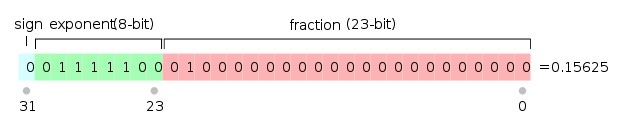
\includegraphics[width=.5\textwidth]{img/IEEE_754_Single_Floating_Point_Format}
\caption{Distribuição dos bits. Precisão simples \cite{wiki:ieee754en}}
\label{fig:ieee754ps}
\end{figure}

A precisão de representação numérica utilizada neste trabalho foi a precisão 
simples. Onde possui 32 bits que em representação seriam 7 digitos decimais.
Destes 32 bits 1 bit é para o sinal, 8 bits para o expoente e 23 bits para 
representar a mantissa.